\documentclass[12pt]{article}
\usepackage[a4paper, portrait, margin=2cm]{geometry}
\usepackage{graphicx} % Required for inserting images
\usepackage[page,toc,titletoc,title]{appendix}
\usepackage{mathptmx}
\usepackage{pdflscape}
\usepackage{pdfpages}
\usepackage{enumitem}
\usepackage{hyperref}
\usepackage{cleveref}
\usepackage{wrapfig}
\usepackage{gensymb}

\title{Surrogate Modelling in a Live Simulation Environment}

\author{Bert Downs }

\date{October 2024}

\begin{document}

\maketitle

Digital Twin technology is seen as transformative in many industries, as they enable new methods of control, optimisation, scheduling, and design~\cite{walmsley2024adaptive}. The increase in efficiency they promise is particularly attractive in the energy sector, where it can reduce both emissions and costs.

Some key technologies underpining digital twins include:

\begin{itemize}
    \item Traditional Process Simulation techniques, where mathematical physics-based models are used to simulate the behaviour of a system \cite{lee2021idaes}.
    \item Data Collection and Processing techniques, such as SCADA systems or Industrial IoT systems, which enable observability and control \cite{udugama2020role},
    \item Physics-Informed Machine Learning, where machine learning models are combined with traditional physics-based models to improve accuracy and generalisation \cite{karniadakis2021physics}.
\end{itemize}

There is a growing body of research into new machine learning techniques that can be used to accurately model complex systems. New fields of machine learning, such as Operator Networks, are particularly promising as they offer the ability to predict the solution to Ordinary Differential Equations (ODEs) and Partial Differential Equations (PDEs)\cite{lu2019deeponet}, which are commonly used in physics-based models.

From a Software Engineering perspective, these techniques exist as research concepts, but there is a gap in the literature on how to implement them in a live industrial environment. This project aims to bridge that gap by developing a framework for implementing these techniques, with industrial chemical processes providing a case study.

\section{Research Questions and their significance}

This project aims to answer the following research questions:

\textbf{RQ1: What adjustments need to be made to existing machine learning techniques to make them suitable for a live ``Digital Twin'' environment?}

Online learning has unique challenges not present in offline learning, because the model must be updated in real-time, meaning that there are strict processing time constraints. Additionally, concept drift can occur, where the underlying system changes over time and the model must adapt to this. This is common in industrial processes, where equipment can degrade over time, or process conditions can change. There is little research into how new machine learning techniques, such as Operator Networks, can be adapted to these constraints.

\textbf{RQ2: How can different fidelity models (including physics-based models, machine learning models, and hybrid models) be combined to create a Digital Twin?} 

Each different modelling technique has different strengths and weaknesses. Physics-based models are accurate, and generalise well, but can be computationally expensive. Machine learning models are often faster, and can easily respond to change, but do not generalise well. In an industrial setting it may be benificial to use different types of models in different circumstances, or to combine them in some way. This research question aims to explore the different ways that models can be combined, from an operational standpoint.


\textbf{RQ3: What software architecture would support this?}

Recent research into advanced modelling and optimisation techniques is more likely to be used if there is a clear path to implementation. This research question will apply software engineering principles to the the findings of RQ1 and RQ2, to develop a platform that supports the implementation of these techniques in an industrial setting. Project Ahuora, a research group in the University of Waikato, is developing an energy-technology platform using process simulation and adaptive digital twin technology. It is being built to support many different types of chemical analysis, reducing redundancy by using the same data structures for each. This project will contribute to the development of the Ahuora platform, by extending it to support dynamic modelling, surrogate modelling, data-driven modelling, optimisation, and control tooling. These workflows will make it simpler for the industry to adopt recent research. The Ahuora platform will be used as a case study to investigate a suitable software architecture, taking into account the needs of relevant stakeholders.

\section{Proposed Methodology}

This project includes a mix of software engineering, data science, and chemical engineering. Much of the novelty in this project comes from combining research from these different fields, to create something that works better in the real world. Thus, a significant amount of time will be spent reviewing relevant literature in these fields, to understand the most recent and most robust techniques available. This research will then be considered in the context of other disciplines, to understand where it can be applied.

Much of the research will be conducted using software engineering principles of development, testing, deployment, and feedback. By iteratively improving the Ahuroa platform, different modelling techniques can be tested and compared. Small-scale experiments, case studies, and prototypes will be used to test the effectiveness of different modelling techniques, and their suitability for a live industrial environment.

Through the initial research, and over time, a better understanding of what is required will be developed. However, an initial roadmap for development has been provided in appendix \ref{sec:roadmap}.

\section{Expected Outcome}

Through this research, it is expected that a framework for implementing advanced machine learning techniques in a live industrial environment will be developed. The Ahuora platform will be extended to support these techniques, and will be used as a case study to demonstrate their effectiveness. This will provide a proof of concept for the use of these techniques in a real-world setting, and will provide a tool for industrial partners to use in their own processes.


% \section{Resources}

% Compute, servers to test on.
% Developers
% Data (from a real industrial process)
% Access to the Ahuora platform


% What background research is there?
% All the live data stuff
% all the idaes stuff
% all the surrogate modelling stuff
% all the physics informed stuff
% all the ahuora stuff

% What can we add?
% operator networks, more physics informed, but also a LIVE SYSTEM UPDATES not just historical data

% What is the plan?

% Ahuora makes a good case study as a plaform with a live simulation enviromnent
% but, we can make a more general solution for operator networks, in mathematical modelling, in live data
% we can also look at operator networks, in live data, which goes to mathematical modelling (no neural networks in the mathematical model)
% or maybe operator networks as a live surrogate of a mathematical model that's too slow to run/update in real time

% We can also look at the physics informed stuff, and how that can be used in a operator network. (?maybe)


%https://www.overleaf.com/learn/latex/Bibtex_bibliography_styles
\bibliographystyle{apalike}
\bibliography{refs} % Entries are in the refs.bib file


\begin{appendices}
    
    
\begin{landscape}
\section{Roadmap} \label{sec:roadmap}
\begin{figure}[h]
    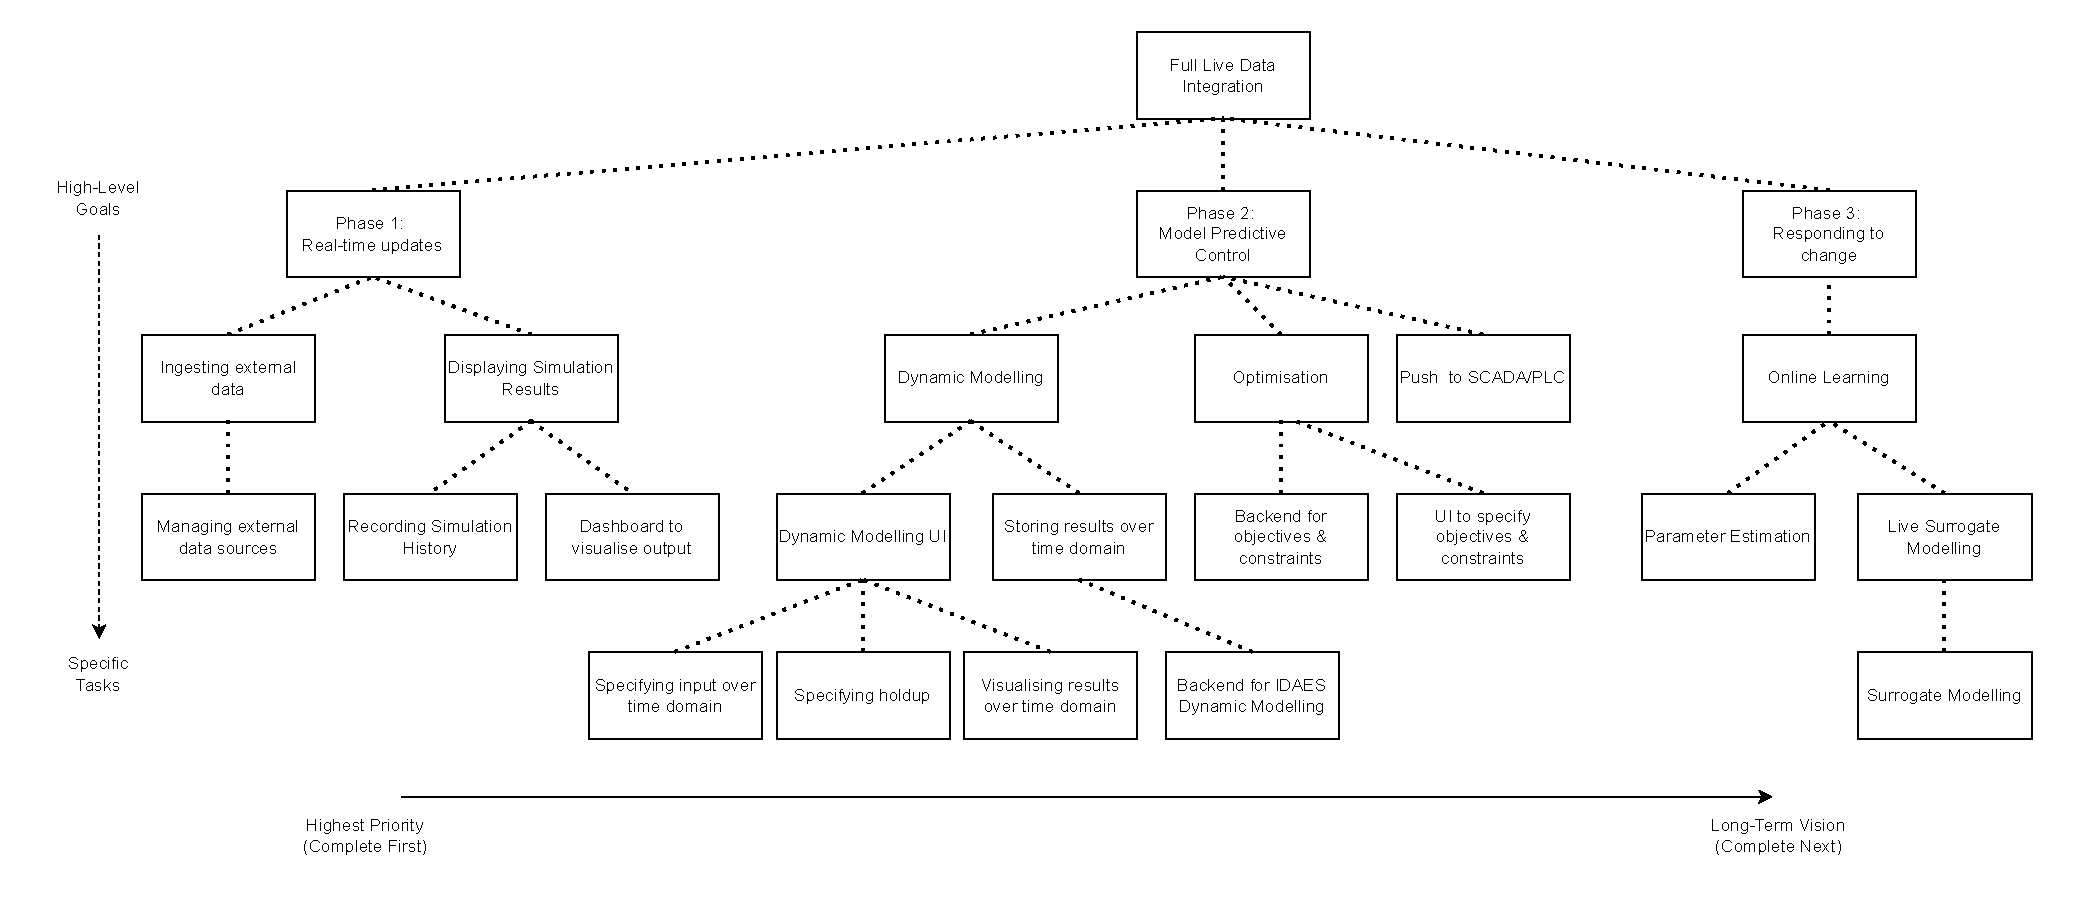
\includegraphics[width=1.5\textwidth]{../roadmap.pdf}
    \caption{Roadmap, showing the initial areas of development of the Ahuora Digital Twin Platform.}
\end{figure}
\end{landscape}

\end{appendices}


\end{document}